% !TeX root = ../../../Main.tex
\chapter{Reinforcement Learning}

\section{Markov Decision Process}

A Markov Decision Process is a series of decision problems, where each decision has an impact on the final reward the agent receives. In an MDP, the probability of reaching a state $s_{t+1}$ by taking an action $a_t$ only depends on the state $s_t$. The predecessor states of $s_t$ are irrelevant for $P(s_{t+1}|s_t,a_t)$.

\begin{align}
P(s',r|s,a)&=\mathbb{P}[s_{t+1}=s',r_{t+1}=r|s_t=s,a_t=a] \\
&= \mathbb{P}[s_{t+1}|s_t,a_t,s_{t-1},a_{t-1},s_{t-2},a_{t-2},...]
\end{align}

In most RL-problems, the goal is to maximize the total return from a given initial state. This is done by trying to find the optimal policy $\pi^*$ which yields the maximum expected return from each state. $\pi^*$ can be achieved directly or by finding the optimal value function, i.e. the mapping from each state or state-action-pair to its true value $V^*$. The definition of a state value is given in section \ref{sec:value-function} If $\pi^*$ is found for a specific MDP, the MDP is solved.

\section{The Agent - Environment System}

In Reinforcement Learning scenarios, an agent interacts with its environment and thereby tries to maximize some sort of reward. By interacting with its environment, it learns how to behave optimally with respect to maximizing a scalar reward signal. The agent aims to maximize its total reward by choosing - at each time step - the best possible action $a$ from a set of actions $\mathcal{A}$. 
The agent has no prior knowledge about the environment and about how to behave in an optimal way. Instead, it learns by interacting with its environment and the information it receives during training. Before each step, the agent is in a state $s_t$, chooses an action $a_t$ and receives a scalar reward $r_t$ and an observation $o_t$ belonging to the next state $s_{t+1}$. The process is repeated, then. Figure \ref{fig:agent_env_system} illustrates what happens at each time step.

The reward $r_t$ the agent receives at each step is determined by a reward function $\mathcal{R}(s,a)$. The choice of a reward function is crucial for the success of any RL-based trajectory optimization algorithm. The only way to "tell" the agent, what his goal is, is by defining the reward function. Generally, a reward function should give the agent a positive reward for actions that bring him closer to his goal and penalize actions that reduce his chances of reaching it. If an action takes the agent to a terminal state that is not the goal, this action should yield a big penalty. Penalties are a means of keeping the agent away from states that are not desirable, such as unwanted terminal states or states in their direct vicinity. More on the reward function used here can be found in chapter \ref{chapter3} 

\begin{figure}[h]
	\centering
	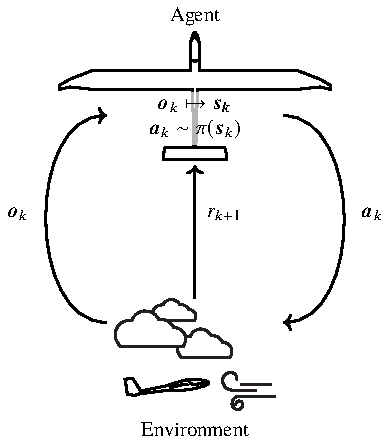
\includegraphics[width=0.5\textwidth]{src/pics/RLProblem.pdf}
	\caption{The Agent-Environment-System \cite{Notter2018}}
	\label{fig:agent_env_system} 
\end{figure}

\section{Model Based and Model Free Learning}

MDP solution methods can be divided into model-free and model-based methods. In model-based methods, the agent uses a model to predict the reaction of the environment to any of his actions. An environment model typically takes a state-action pair and returns the next state and next reward. If the environment is stochastic, there are multiple possible next states and rewards. A \textit{sample model} returns one of the possibilities, whereas a \textit{distribution model} returns some representation of all possible next states and rewards.

Regardless of the type, all models approximate what might happen to the agent in future time steps. Whether the experience gathered through a model is useful obviously depends on its quality. To distinguish experience from a model from real experience, the results from a model are referred to as \textit{simulated experience}\cite{SuttonBarto2018}. Figure \ref{fig:model-based-model-free} shows some popular Machine Learning algorithms and classifies them.

\section{Agent}

The agent in an MDP consists of at least one of the following parts.

\begin{itemize}
	\item Policy: \\
	A mapping from states to actions that tells the agent what to do (c.f. section \ref{sec:policy})
	\item Value Function: \\
	A mapping from states (or state-action pairs) to values (c.f. section \ref{sec:value-function})
	\item Model: \\
	A model of the environment that might be updated by the agent's experience
\end{itemize}

Most agents have a policy. They also can have a value function, like in actor-critic algorithms where the value function is used for bootstrapping. This means utilizing the Bellman Expectation Equation to estimate the return $G_t$ by doing a one step lookahead and use the sum of the immediate reward and the successor state value.

\begin{align}
\mathbb{E}[G_t|s_t=s] &= \mathbb{E}[R_{t+1} + \gamma G_{t+1}|s_t=s, a_t=a] \\
&=\mathbb{E}[R_{t+1}+ \gamma V(s_{t+1})|s_t=s, a_t=a]
\end{align}

Instead of sampling a complete episode, bootstrapping makes it possible to learn from incomplete episodes.

A model of the environment is - in principle - not required for successful training. It can however be used to gather simulated experience and therefore reduce training time on a real agent like a robot. Although imperfect, information from a model can be useful in such cases where training time is restricted which particularly holds true for robots flying outdoors.

\section{Return}

The return $G_t$ at a time step $t$ is the cumulative reward $r_t$ at each step from the state $s_t$ onwards until reaching a terminal state:

\begin{equation}
G_t = \sum_{k=0}^{T-t-1}\gamma^k r_{t+k+1}
\end{equation}

If $\gamma \in (0,1]$ is close to zero, immediate rewards are weighted stronger. If $\gamma$ is close to one, rewards in the distant future are weighted likewise, making decisions more far sighted. In infinite horizon problems where there is no terminal state, $\gamma$ must be less than one in order to avoid infinite returns. In finite horizon (i.e. episodic) MDPs, $\gamma$ is usually close to, or exactly one.

Each decision at a given state $s_t$ also affects what the next state $s_{t+1}$ is and therefore the next reward. More on the reward and what role it plays in Dynamic Programming is explained in section \ref{sec:reward}

\section{Policy}
\label{sec:policy}
In reinforcement learning problems, a policy is usually the part that represents the agent. It contains all the information needed to decide what action to choose in each state the agent visits. A policy is a mapping from states to actions.

\begin{equation}
\pi: \mathcal{S} \times \mathcal{A} \mapsto [0,1]
\end{equation} 

The policy is a probability distribution over actions given states and returns - for each state - the probability of taking an action $a_t$. If the policy is deterministic, only one $a_t$ out of $\mathcal{A}$ has a probability of one with all other actions assigend to probability zero. In any policy, the sum of all possible action-probabilities must be one.

\begin{equation}
\pi(a|s) = \mathbb{P}[a_t=a|s_t=s]
\end{equation}

This yields equations \ref{eq:transprobpi} and \ref{eq:rewardpi} for the state transition probability and the reward function under policy $\pi$. The reward function is explained in section \ref{sec:reward-function}.

\begin{equation}
\mathcal{P}^\pi(s,s')=\sum_a \pi(a|s)\mathcal{P}(s'|s,a)
\label{eq:transprobpi}
\end{equation}
\begin{equation}
\mathcal{R}^\pi(s) = \sum_a\pi(a|s)\mathcal{R}(s,a)
\label{eq:rewardpi}
\end{equation}

At each timestep, the agent receives a state observation $o_{t-1}$ from the environment, passes it to the policy and the policy returns an action $a_t$. This action is taken and the agent gets a new observation $o_t$ and a reward $r_t$. This process is repeated until the agent reaches a terminal state.

A policy can be implemented in many different ways. The simplest option is a table where each field contains the action for one state or - if the policy is stochastic - all possible actions and their respective probabilities. Other examples include linear combinations of the inputs and linear combinations of basis functions. The most popular way to implement a policy is - however - through an artificial neural network (ANN). More information about neural networks is given in chapter \ref{chapter3}.  

\section{Value Functions}
\label{sec:value-function}

Some RL-algorithms try to find a policy directly from experience. Others, like Q-learning, additionally utilize a so called value function. A value function maps from states or state-action pairs to their values. In this context, the value of a state or an action is a measure of how useful it is for the agent to visit the respective state or choosing the respective action. There are two types of value functions, state value functions and action value functions. The state value $V(s)$ is the expected total return from state $s_t$ onwards until the episode terminates. The action value also takes into account what the agent chooses to do in state $s_t$. It is the expected total return from state $s_t$ when choosing action $a_t$.

\begin{equation}
V(s) = \mathbb{E}[G_t|s_t=s]
\label{eq:state_value_fun}
\end{equation}

\begin{equation}
Q(a|s) = \mathbb{E}[G_t|s_t=s,a_t=a]
\label{eq:action_value_fun}
\end{equation}

In the following sections, the action space is regarded finite for simplicity.
The state value function \ref{eq:state_value_fun} can be expressed in terms of the action value function \ref{eq:action_value_fun}:

\begin{equation}
V_\pi(s) = \sum_{a}\pi(a|s)Q_\pi(s,a)
\label{eq:state_value_function_with_q}
\end{equation}

Similarly, the action value function can be expressed by means of the state value function:

\begin{equation}
Q_\pi(s,a)=\mathcal{R}(s,a)+\gamma \sum_{s'}\mathcal{P}(s'|s,a)V_\pi(s')
\label{eq:action_value_function_with_v}
\end{equation}

If an agent has found the optimal value function $V^*$ or $Q^*$ of an MDP, the optimal policy $\pi^*$ can be derived directly by acting greedily with respect to the value function at each state.

Like a policy, a value function may be implemented as a table, a linear combination of the input features, a combination of basis functions, or an artificial neural network.

\section{The Bellman Expectation Equation}

According to the Bellman Expectation Equation, every trajectory through the state space can be decomposed into two parts: the next step and the rest of the path. Equivalently, every state value can be split into the value of the next step and the successor state value.

The state value function \ref{eq:state_value_fun} can be written as a weighted sum of the action values, each multiplied with the probability to take the respective action according to the policy. Replacing $Q_\pi(s,a)$ in equation \ref{eq:state_value_function_with_q} with equation \ref{eq:action_value_function_with_v} yields equation \ref{eq:bellman_exp_eq_V_Q} which is known as the \textit{Bellman Expectation Equation}:
\begin{align}
V_\pi(s)&=\sum_a \pi(a|s)Q_\pi(s,a)\\ &= \sum_a \pi(a|s)\sum_r \sum_{s'} \mathcal{P}(s',r|s,a)[r+\gamma V_{\pi}(s')]
\label{eq:bellman_exp_eq_V_Q}
\end{align}

In a deterministic environment, equation \ref{eq:bellman_exp_eq_V_Q} becomes

\begin{equation}
V_\pi(s)= \sum_a \pi(a|s)[r+\gamma V_{\pi}(s')]
\label{eq:bellman_exp_eq_V_determinisic}
\end{equation}

The Bellman Expectation Equation can be used to update a state value by looking at the state values of its successor states and weighting them by the probabilities to reach each successor state (c.f. equations \ref{eq:bellman_exp_update_bootstrapped} and \ref{eq:bellman_exp_update_discrete}).

\section{The Bellman Optimality Equation}

Instead of a weighted sum of rewards and successor values, like in equation \ref{eq:bellman_exp_eq_V_Q}, one can take only the action that has the maximum action value. This yields the following equation:

\begin{align}
V_*(s)&=\max_{a \in \mathcal{A}(s)} Q_{\pi_*}(s,a) \label{eq:bellman_optimality_equation_v_with_q}\\
&=\max_{a}\mathbb{E}_{\pi_*}[G_t|s_t=s,a_t=a]\\
&=\max_{a}\mathbb{E}_{\pi_*}[R_{t+1} + \gamma G_{t+1}|s_t=s,a_t=a]\\
&=\max_{a}\mathbb{E}[R_{t+1} + \gamma V_*(s_{t+1})|s_t=s,a_t=a]\\
&=\max_{a}\sum_{s',r}\mathcal{P}(s',r|s,a)[r + \gamma V_*(s')]
\label{eq:bellman_optimality_equation_stochastic}
\end{align}

Again, if the environment is deterministic, equation \ref{eq:bellman_optimality_equation_stochastic} can be simplified:

\begin{equation}
V_*(s) = \max_a[r+\gamma V_*(s')]
\label{eq:bellman_optimality_equation_deterministic}
\end{equation}

All equations from \ref{eq:bellman_optimality_equation_v_with_q} to \ref{eq:bellman_optimality_equation_deterministic} are alternative ways to express the \textit{Bellman Optimality Equation}. It states that the value of a state under an optimal policy must equal the expected return for the best action in that state \cite{SuttonBarto2018}. Intuitively it is obvious that the optimal policy must pick the best action in each state. In Value Iteration, the \textit{Bellman Optimality Equation} is used as an update rule. See chapter \ref{subsection:VI} for more details.